% Copyright (C) 2005-2015 Airbus - EDF - IMACS - Phimeca
% Permission is granted to copy, distribute and/or modify this document
% under the terms of the GNU Free Documentation License, Version 1.2
% or any later version published by the Free Software Foundation;
% with no Invariant Sections, no Front-Cover Texts, and no Back-Cover
% Texts.  A copy of the license is included in the section entitled "GNU
% Free Documentation License".
\renewcommand{\filename}{docUC_StocProc_BoxCox.tex}
\renewcommand{\filetitle}{UC : Box Cox transformation}

% \HeaderNNIILevel
% \HeaderIILevel
\HeaderIIILevel

\label{BoxCox}

\index{Stochastic Process! Box Cox}

The objective of this Use Case  is to estimate a Box Cox transformation from a field which all values are positive (eventually after a shift to satisfy the positiveness) and to apply it on the field.\\

We consider $X: \Omega \times \cD \rightarrow \Rset^d$ a multivariate stochastic process of dimension $d$ where $\cD \in \Rset^n$ and $\omega \in \Omega$ is an event. We suppose that the process is  $\cL^2(\Omega)$.\\
We note $X_{\vect{t}}: \Omega \rightarrow \Rset^d$ the random variable at the vertex $\vect{t} \in \cD$ defined by $X_{\vect{t}}(\omega)=X(\omega, \vect{t})$.\\

If the variance  of $X_{\vect{t}}$ depends on the vertex $\vect{t}$, the Box Cox transformation maps the process $X$ into the process $Y$ such that the variance of $Y_{\vect{t}}$ is constant (at the first order at least) with respect to $\vect{t}$.\\

We present here :
\begin{itemize}
\item the estimation of the Box Cox transformation from a given field of the process $X$,
\item the action of the Box Cox transformation on a field generated from $X$.
\end{itemize}

We note $h: \Rset^d \rightarrow \Rset^d$ the Box Cox transformation which maps the process $X$ into the process $Y: \Omega \times \cD \rightarrow \Rset^d$, where $Y=h(X)$, such that  $\Var{Y_{\vect{t}}}$ is independent of $\vect{t}$ at the first order.\\
We suppose that $X_{\vect{t}}$ is a positive random variable for any $\vect{t}$. To verify that constraint, it may be needed to consider the shifted process $X+\vect{\alpha}$. \\

We illustrate some usual Box Cox transformations $h$ in the scalar case ($d$=1), using the Taylor development of $h: \Rset \rightarrow \Rset$ at the mean point of  $X_{\vect{t}}$. \\
In the mutlivariate case, we estimate the Box Cox transformation component by component and we define the multivariate Box Cox transformation as the aggregation of the marginal Box Cox transformations.\\

{\bf Marginal Box Cox tranformation: }\\
The first order Taylor development of $h$ around $\Expect{Y_{\vect{t}}}$ writes:
\begin{eqnarray*}
  \forall \vect{t} \in \cD, h(X_{\vect{t}}) & = & h(\Expect{X_{\vect{t}}}) + (X_{\vect{t}} - \Expect{X_{\vect{t}}})h'(\Expect{X_{\vect{t}}})
\end{eqnarray*}
which leads to:
\begin{eqnarray*}
  \Expect{h(X_{\vect{t}})} & = & h(\Expect{X_{\vect{t}}})
\end{eqnarray*}
and then:
\begin{eqnarray*}
  \Var{h(X_{\vect{t}})} & = & h'(\Expect{X_{\vect{t}}})^2  \Var{X_{\vect{t}}}
\end{eqnarray*}



To have $ \Var{h(X_{\vect{t}})}$ constant with respect to $\vect{t}$ at the first order, we need :
\begin{eqnarray}\label{eqh}
  h'(\Expect{X_{\vect{t}}}) = k \left(  \Var{X_{\vect{t}}} \right)^{-1/2}
\end{eqnarray}

Now, we make some additional hypotheses on the relation between $\Expect{X_{\vect{t}}}$ and $\Var{X_{\vect{t}}}$ :
\begin{itemize}
\item If we suppose that  $\Var{X_{\vect{t}}} \propto \Expect{X_{\vect{t}}}$,  then (\ref{eqh}) leads to the function $h(y) \propto \sqrt{y}$ and we take $h(y) = \sqrt{y}, y~>~0$;
\item If we suppose that $\Var{X_{\vect{t}}} \propto (\Expect{X_{\vect{t}}})^2$ , then  (\ref{eqh}) leads to the function $h(y) \propto \log{y}$ and we take $h(y) = \log{y}, y>0$;
\item More generally, if we suppose that $\Var{X_{\vect{t}}} \propto (\Expect{X_{\vect{t}}})^{\beta}$, then (\ref{eqh}) leads to the function $h_\lambda$ parametered by the scalar $\lambda$ :

  \begin{eqnarray}
    \label{BoxCoxModel}
    h_\lambda(y) & = &
    \left\{
    \begin{array}{ll}
      \frac{y^\lambda-1}{\lambda} & \lambda \neq 0 \\
      \log(y)                      & \lambda = 0
    \end{array}
    \right.
  \end{eqnarray}
  where $\lambda = 1-\frac{\beta}{2}$.
\end{itemize}

The inverse Box Cox transformation is defined by:
\begin{eqnarray}
  \label{InverseBoxCoxModel}
  h^{-1}_\lambda(y) & = &
  \left\{
  \begin{array}{ll}
    \displaystyle (\lambda y + 1)^{\frac{1}{\lambda}} & \lambda \neq 0 \\
    \displaystyle \exp(y)                          & \lambda = 0
  \end{array}
  \right.
\end{eqnarray}
\vspace*{0.1cm}

{\bf Estimation of the Box Cox tranformation: }\\
The parameter $\lambda$ is estimated from a given field of the process $X$ as follows.\\
The estimation of $\lambda$ given below is optimized in the case when $h_\lambda(X_{\vect{t}}) \sim \cN(\beta , \sigma^2 )$ at each vertex $\vect{t}$. If it is not the case, that estimation can be considered as a proposition, with no garantee.\\
The parameters $(\beta,\sigma,\lambda)$ are then estimated by the maximum likelihood estimators. We note $\Phi_{\beta, \sigma}$ and $\phi_{\beta, \sigma}$ respectively the cumulative distribution function and the density probability function of the $\cN(\beta , \sigma^2)$ distribution.\\
For all vertices $\vect{t}$, we have :
\begin{eqnarray}\label{cdfYt}
  \forall v \geq 0, \, \Prob{ X_{\vect{t}} \leq v } & = & \Prob{ h_\lambda(X_{\vect{t}}) \leq h_\lambda(v) } \\
  & = & \Phi_{\beta, \sigma} \left(h_\lambda(v)\right)
\end{eqnarray}

from which we derive the  density probability function $p$ of $X_{\vect{t}}$ for all vertices $\vect{t}$ :
\begin{eqnarray}\label{pdfYt}
  p(v) & = & h_\lambda'(v)\phi_{\beta, \sigma}(v) = v^{\lambda - 1}\phi_{\beta, \sigma}(v)
\end{eqnarray}
Using (\ref{pdfYt}), the likelihood of the values $(x_0, \dots, x_{N-1})$ with respect to the model (\ref{cdfYt})  writes:
\begin{eqnarray}\label{LKH}
  L(\beta,\sigma,\lambda)
  & = &
  \underbrace{ \frac{1}{(2\pi)^{N/2}}
    \times
    \frac{1}{(\sigma^2)^{N/2}}
    \times
    \exp\left[
      -\frac{1}{2\sigma^2}
      \sum_{k=0}^{N-1}
      \left(
      h_\lambda(x_k)-\beta
      \right)^2
      \right]
  }_{\Psi(\beta, \sigma)}
  \times
  \prod_{k=0}^{N-1} x_k^{\lambda - 1}
\end{eqnarray}



We notice that for each fixed $\lambda$, the likelihood equation is proportional to the likelihood equation which estimates  $(\beta, \sigma^2)$.
Thus, the maximum likelihood estimator for $(\beta(\lambda), \sigma^2(\lambda))$ for a given $\lambda$  are :
\begin{eqnarray}\label{eqBetaSigma}
  \hat{\beta}(\lambda) & = & \frac{1}{N} \sum_{k=0}^{N-1} h_{\lambda}(x_k) \\
  \hat{\sigma}^2(\lambda)  & = &  \frac{1}{N} \sum_{k=0}^{N-1} (h_{\lambda}(x_k) - \beta(\lambda))^2
\end{eqnarray}

Substituting (\ref{eqBetaSigma}) into (\ref{LKH}) and taking the $\log-$likelihood, we obtain :
\begin{eqnarray}\label{lLambda}
  \ell(\lambda) = \log L( \hat{\beta}(\lambda), \hat{\sigma}(\lambda),\lambda ) & = & C -
  \frac{N}{2}
  \log\left[\hat{\sigma}^2(\lambda)\right]
  \;+\;
  \left(\lambda - 1 \right) \sum_{k=0}^{N-1} \log(x_i)\,,%\qquad mbox{where $C$ is a constant.}
\end{eqnarray}
The parameter $\hat{\lambda}$ is the one maximising $\ell(\lambda)$ defined in (\ref{lLambda}).\\


{\bf OpenTURNS objects}:\\
The OpenTURNS object \emph{BoxCoxFactory} enables to create a factory of Box Cox transformation.\\

Then, OpenTURNS estimates the Box Cox transformation $h_{\vect{\lambda}}$ from  the initial field values $(\vect{x}_0, \dots, \vect{x}_{N-1})$ thanks to the method \emph{build} of the object \emph{BoxCoxFactory}, which produces an object of type \emph{BoxCoxTransform}. \\

If the field values  $(\vect{x}_0, \dots, \vect{x}_{N-1})$ have some negative values, it is possible to translate the values with respect a given shift $\vect{\alpha}$ which has to be mentionned either at the creation of the object {\itshape BoxCoxFactory} or when using the method \emph{build}.\\
Then the  Box Cox transformation is the composition of $h_{\vect{\lambda}}$  and this translation. \\


The object \emph{BoxCoxTransform} enables to :
\begin{itemize}
\item  transform the field values  $(\vect{x}_{0}, \dots,\vect{x}_{N-1})$ of dimension $d$ into the values $(\vect{y}_{0}, \dots, \vect{y}_{N-1})$  with stabilized variance, such that for each vertex $\vect{t}_i$ we have:
  \begin{equation}\label{Eval}
    \vect{y}_{i} = h_{\vect{\lambda}}(\vect{x}_{i})
  \end{equation}
  or
  \begin{equation}
    \vect{y}_{i} = h_{\vect{\lambda}}(\vect{x}_{i} + \vect{\alpha})
  \end{equation}
  thanks to the operand  \emph{()}. The field based on the values $\vect{y}_{i}$ shares the same mesh than the initial field.
\item create the inverse Box Cox transformation such that :
  \begin{equation}
    \vect{x}_{i}= h^{-1}_{\vect{\lambda}}(\vect{y}_{i} )
  \end{equation}
  or
  \begin{equation}
    \vect{x}_{i} = h^{-1}_{\vect{\lambda}}(\vect{y}_{i} ) - \vect{\alpha}
  \end{equation}
  thanks to the method \emph{getInverse()} which produces an object of type \emph{InverseBoxCoxTransform} that can be evaluated on a field thanks to the operator  \emph{()}. The new field based  shares the same mesh than the initial field.
\end{itemize}



\requirements{

  \begin{description}
  \item[$\bullet$] somefields: {\itshape myField}
  \item[type:]  Field
  \end{description}

  \begin{description}
  \item[$\bullet$] $\vect{\lambda}$: {\itshape myLambda}
  \item[type:]  NumericalPoint
  \end{description}

}
{
  \begin{description}
  \item[$\bullet$] a Box Cox factory: {\itshape myBoxCoxFactory }
  \item[type:]  BoxCoxFactory
  \end{description}

  \begin{description}
  \item[$\bullet$] a Box Cox transformation and its inverse: {\itshape myModelTranform, myInverseModelTransform}
  \item[type:]  BoxCoxTransform, InverseBoxCoxTransform
  \end{description}


  \begin{description}
  \item[$\bullet$] $\vect{\lambda}$: {\itshape estimatedLambda}
  \item[type:]  NumericalPoint
  \end{description}


  \begin{description}
  \item[$\bullet$] some mapped fields: {\itshape myStabilizedField}
  \item[type:]  Field
  \end{description}
}

\textspace\\
Python script for this Use Case :

\inputscript{script_docUC_StocProc_BoxCox}


Consider the temporal normal process of dimension~1 which covariance model is $Exponential(a,\lambda)$ with $(a, \lambda)=(1.0, 0.2)$ and which  bidimensional mesh is the box $[0,2]\times [0,1]$ regularly discretized with 40 points in the first dimension and 20 points in the second one. \\
Then we map this process $X$ into the process $Y=\exp(X)$ in order to get a non stationary  positive process.\\
Then we get a field generated by the process $Y$ and we apply the Box Cox transformation. Figures \ref{InitField} and  \ref{StabField} respectively draw the initial field and the stabilized one. We note that the variations in the values have decreased (colors are more uniform after the Box Cox transformation). The associated $\lambda\simeq 0$.

\begin{figure}[H]
  \begin{minipage}{9cm}
    \begin{center}
      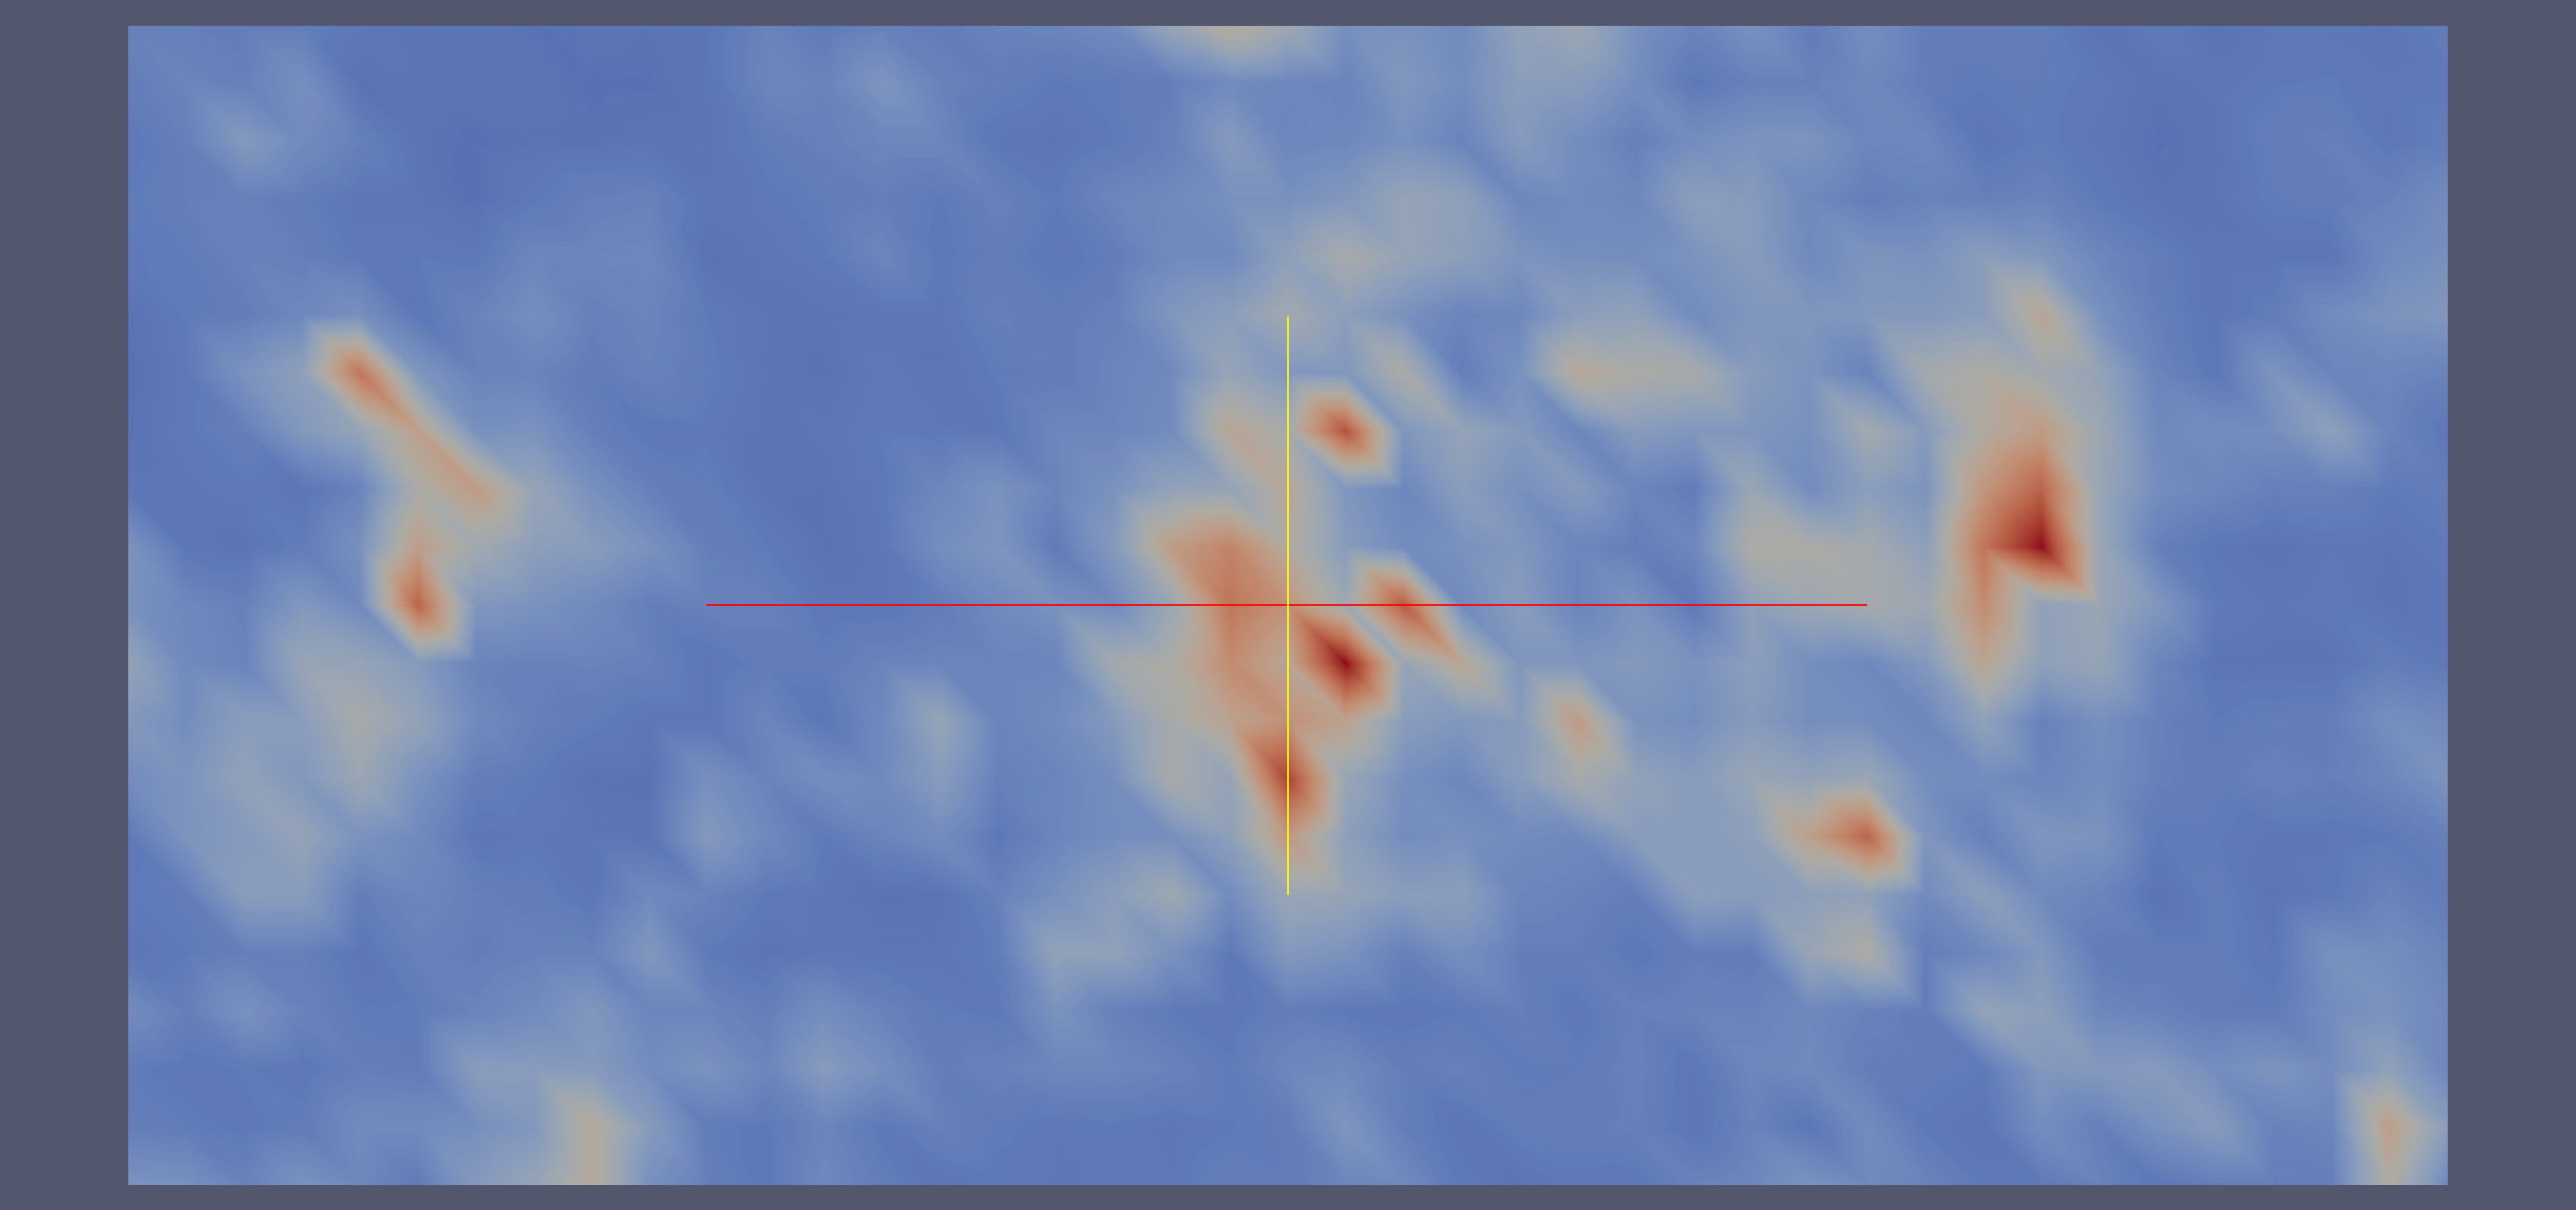
\includegraphics[width=9cm]{Figures/BoxCoxInitField.pdf}
      \caption{One field from the Y process.}
      \label{InitField}
    \end{center}
  \end{minipage}
  \hfill
  \begin{minipage}{9cm}
    \begin{center}
      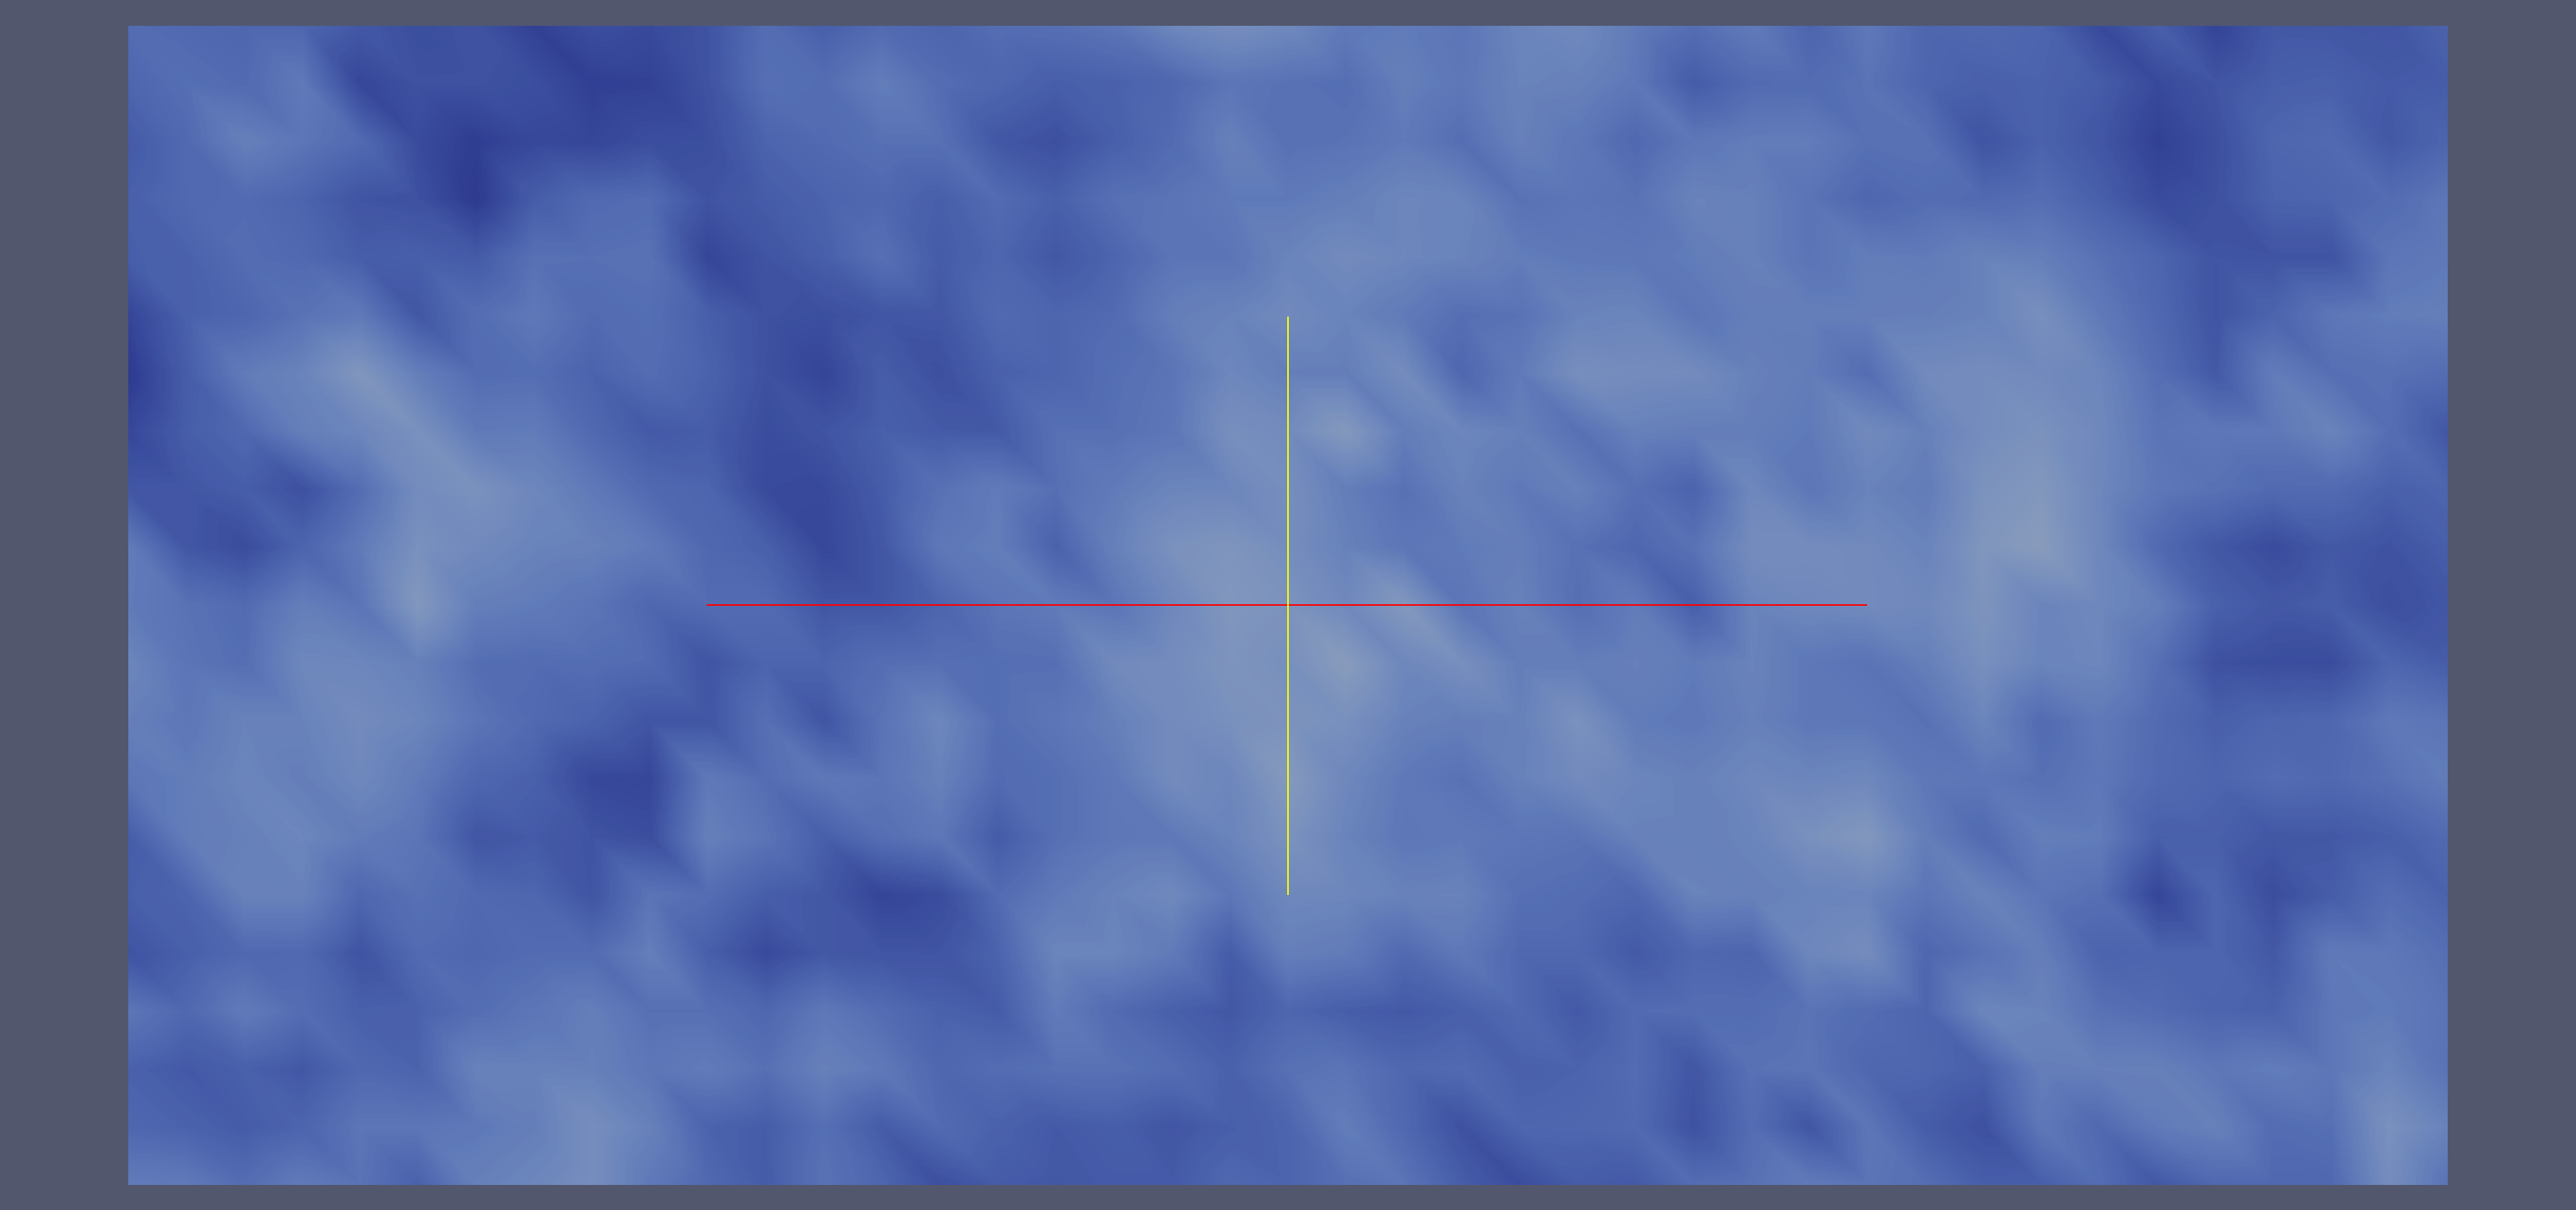
\includegraphics[width=9cm]{Figures/BoxCoxStabilizedField.pdf}
      \caption{Field of Figure \ref{InitField} after the Box Cox transformation.}
      \label{StabField}
    \end{center}
  \end{minipage}
\end{figure}
